%%% The main file. It contains definitions of basic parameters and includes all other parts.

%% Settings for single-side (simplex) printing
% Margins: left 40mm, right 25mm, top and bottom 25mm
% (but beware, LaTeX adds 1in implicitly)
\documentclass[12pt,a4paper]{report}
\setlength\textwidth{145mm}
\setlength\textheight{247mm}
\setlength\oddsidemargin{15mm}
\setlength\evensidemargin{15mm}
\setlength\topmargin{0mm}
\setlength\headsep{0mm}
\setlength\headheight{0mm}
% \openright makes the following text appear on a right-hand page
\let\openright=\clearpage

%% Settings for two-sided (duplex) printing
% \documentclass[12pt,a4paper,twoside,openright]{report}
% \setlength\textwidth{145mm}
% \setlength\textheight{247mm}
% \setlength\oddsidemargin{14.2mm}
% \setlength\evensidemargin{0mm}
% \setlength\topmargin{0mm}
% \setlength\headsep{0mm}
% \setlength\headheight{0mm}
% \let\openright=\cleardoublepage

%% Generate PDF/A-2u
\usepackage[a-2u]{pdfx}

%% Character encoding: usually latin2, cp1250 or utf8:
\usepackage[utf8]{inputenc}

%% Prefer Latin Modern fonts
\usepackage{lmodern}

%% Further useful packages (included in most LaTeX distributions)
\usepackage{amsmath}        % extensions for typesetting of math
\usepackage{amsfonts}       % math fonts
\usepackage{amsthm}         % theorems, definitions, etc.
\usepackage{bbding}         % various symbols (squares, asterisks, scissors, ...)
\usepackage{bm}             % boldface symbols (\bm)
\usepackage{graphicx}       % embedding of pictures
\usepackage{fancyvrb}       % improved verbatim environment
\usepackage{natbib}         % citation style AUTHOR (YEAR), or AUTHOR [NUMBER]
\usepackage[nottoc]{tocbibind} % makes sure that bibliography and the lists
			    % of figures/tables are included in the table
			    % of contents
\usepackage{dcolumn}        % improved alignment of table columns
\usepackage{booktabs}       % improved horizontal lines in tables
\usepackage{paralist}       % improved enumerate and itemize
\usepackage{xcolor}         % typesetting in color

\usepackage{pdfpages} % MY PACKAGE: inserting other pdf pages

%%% Basic information on the thesis

% Thesis title in English (exactly as in the formal assignment)
\def\ThesisTitle{Semi-supervised learning in Optical Music Recognition}

% Author of the thesis
\def\ThesisAuthor{Jiří Mayer}

% Year when the thesis is submitted
\def\YearSubmitted{2022}

% Name of the department or institute, where the work was officially assigned
% (according to the Organizational Structure of MFF UK in English,
% or a full name of a department outside MFF)
\def\Department{Institute of Formal and Applied Linguistics}

% Is it a department (katedra), or an institute (ústav)?
\def\DeptType{Department}

% Thesis supervisor: name, surname and titles
\def\Supervisor{doc. RNDr. Pavel Pecina, Ph.D.}

% Supervisor's department (again according to Organizational structure of MFF)
\def\SupervisorsDepartment{Institute of Formal and Applied Linguistics}

% Study programme and specialization
\def\StudyProgramme{Computer Science - Software and Data Engineering (N0613A140015)}
\def\StudyBranch{Computer Science - Software and Data Engineering}

% An optional dedication: you can thank whomever you wish (your supervisor,
% consultant, a person who lent the software, etc.)
\def\Dedication{%
Dedication.
}

% Abstract (recommended length around 80-200 words; this is not a copy of your thesis assignment!)
\def\Abstract{%
Optical music recognition (OMR) is a niche subfield of computer vision, where some labeled datasets exist, but there is an order of magnitude more unlabeled data available. Recent advances in the field happened largely thanks to the adoption of deep learning. However, these neural networks are being trained using labeled data only. Semi-supervised learning is a set of techniques that aim to incorporate unlabeled data during training to produce more capable models. We have modified a state-of-the-art object detection architecture and designed a semi-supervised training scheme to utilize unlabeled data. These modifications have successfully allowed us to train the architecture in an unsupervised setting, and our semi-supervised experiments indicate improvements to training stability and reduced overfitting.
}

% 3 to 5 keywords (recommended), each enclosed in curly braces
\def\Keywords{%
{optical music recognition}, {semi-supervised learning}, {deep neural network}
}

%% The hyperref package for clickable links in PDF and also for storing
%% metadata to PDF (including the table of contents).
%% Most settings are pre-set by the pdfx package.
\hypersetup{unicode}
\hypersetup{breaklinks=true}

% Definitions of macros (see description inside)
%%% This file contains definitions of various useful macros and environments %%%
%%% Please add more macros here instead of cluttering other files with them. %%%

%%% Minor tweaks of style

% These macros employ a little dirty trick to convince LaTeX to typeset
% chapter headings sanely, without lots of empty space above them.
% Feel free to ignore.
\makeatletter
\def\@makechapterhead#1{
  {\parindent \z@ \raggedright \normalfont
   \Huge\bfseries \thechapter. #1
   \par\nobreak
   \vskip 20\p@
}}
\def\@makeschapterhead#1{
  {\parindent \z@ \raggedright \normalfont
   \Huge\bfseries #1
   \par\nobreak
   \vskip 20\p@
}}
\makeatother

% This macro defines a chapter, which is not numbered, but is included
% in the table of contents.
\def\chapwithtoc#1{
\chapter*{#1}
\addcontentsline{toc}{chapter}{#1}
}

% Draw black "slugs" whenever a line overflows, so that we can spot it easily.
\overfullrule=1mm

%%% Macros for definitions, theorems, claims, examples, ... (requires amsthm package)

\theoremstyle{plain}
\newtheorem{thm}{Theorem}
\newtheorem{lemma}[thm]{Lemma}
\newtheorem{claim}[thm]{Claim}

\theoremstyle{plain}
\newtheorem{defn}{Definition}

\theoremstyle{remark}
\newtheorem*{cor}{Corollary}
\newtheorem*{rem}{Remark}
\newtheorem*{example}{Example}

%%% An environment for proofs

\newenvironment{myproof}{
  \par\medskip\noindent
  \textit{Proof}.
}{
\newline
\rightline{$\qedsymbol$}
}

%%% An environment for typesetting of program code and input/output
%%% of programs. (Requires the fancyvrb package -- fancy verbatim.)

\DefineVerbatimEnvironment{code}{Verbatim}{fontsize=\small, frame=single}

%%% The field of all real and natural numbers
\newcommand{\R}{\mathbb{R}}
\newcommand{\N}{\mathbb{N}}

%%% Useful operators for statistics and probability
\DeclareMathOperator{\pr}{\textsf{P}}
\DeclareMathOperator{\E}{\textsf{E}\,}
\DeclareMathOperator{\var}{\textrm{var}}
\DeclareMathOperator{\sd}{\textrm{sd}}

%%% Transposition of a vector/matrix
\newcommand{\T}[1]{#1^\top}

%%% Various math goodies
\newcommand{\goto}{\rightarrow}
\newcommand{\gotop}{\stackrel{P}{\longrightarrow}}
\newcommand{\maon}[1]{o(n^{#1})}
\newcommand{\abs}[1]{\left|{#1}\right|}
\newcommand{\dint}{\int_0^\tau\!\!\int_0^\tau}
\newcommand{\isqr}[1]{\frac{1}{\sqrt{#1}}}

%%% Various table goodies
\newcommand{\pulrad}[1]{\raisebox{1.5ex}[0pt]{#1}}
\newcommand{\mc}[1]{\multicolumn{1}{c}{#1}}


% Title page and various mandatory informational pages
\begin{document}
%%% Title page of the thesis and other mandatory pages

%%% Title page of the thesis

\pagestyle{empty}
\hypersetup{pageanchor=false}
\begin{center}

\centerline{\mbox{
\includegraphics[width=166mm]{../img/logo-en.pdf}}}

\vspace{-8mm}
\vfill

{\bf\Large MASTER THESIS}

\vfill

{\LARGE\ThesisAuthor}

\vspace{15mm}

{\LARGE\bfseries\ThesisTitle}

\vfill

\Department

\vfill

{
\centerline{\vbox{\halign{\hbox to 0.45\hsize{\hfil #}&\hskip 0.5em\parbox[t]{0.45\hsize}{\raggedright #}\cr
Supervisor of the master thesis:&\Supervisor \cr
\noalign{\vspace{2mm}}
Study programme:&\StudyProgramme \cr
\noalign{\vspace{2mm}}
Study branch:&\StudyBranch \cr
}}}}

\vfill

% Zde doplňte rok
Prague \YearSubmitted

\end{center}

\newpage

%%% Here should be a bound sheet included -- a signed copy of the "master
%%% thesis assignment". This assignment is NOT a part of the electronic
%%% version of the thesis. DO NOT SCAN.

%%% A page with a solemn declaration to the master thesis

\openright
\hypersetup{pageanchor=true}
\pagestyle{plain}
\pagenumbering{roman}
\vglue 0pt plus 1fill

\noindent
I declare that I carried out this master thesis independently, and only with the cited
sources, literature and other professional sources. It has not been used to obtain another
or the same degree.

\medskip\noindent
I understand that my work relates to the rights and obligations under the Act No.~121/2000 Sb.,
the Copyright Act, as amended, in particular the fact that the Charles
University has the right to conclude a license agreement on the use of this
work as a school work pursuant to Section 60 subsection 1 of the Copyright~Act.

\vspace{10mm}

\hbox{\hbox to 0.5\hsize{%
In \hbox to 6em{\dotfill} date \hbox to 6em{\dotfill}
\hss}\hbox to 0.5\hsize{\dotfill\quad}}
\smallskip
\hbox{\hbox to 0.5\hsize{}\hbox to 0.5\hsize{\hfil Author's signature\hfil}}

\vspace{20mm}
\newpage

%%% Dedication

\openright

\noindent
\Dedication

\newpage

%%% Mandatory information page of the thesis

\openright

\vbox to 0.5\vsize{
\setlength\parindent{0mm}
\setlength\parskip{5mm}

Title:
\ThesisTitle

Author:
\ThesisAuthor

\DeptType:
\Department

Supervisor:
\Supervisor, \SupervisorsDepartment

Abstract:
\Abstract

Keywords:
\Keywords

\vss}

\newpage

\openright
\pagestyle{plain}
\pagenumbering{arabic}
\setcounter{page}{1}


%%% A page with automatically generated table of contents of the master thesis

\tableofcontents

%%% Each chapter is kept in a separate file
\chapter{Introduction}
\label{chap:Introduction}

Optical music recognition (OMR) is the task of extracting semantic information from scans and photos of sheet music. It is a subfield of computer vision, however, traditional computer vision methods are struggling with it unsuccessfully. Especially in the subfield of handwritten music recognition (HMR), where the large variability of handwriting styles poses a great challenge for any handcrafted recognition system. For this reason, recent advances in the field have been made mainly due to the adoption of deep learning. OMR is also a relatively niche field, studied by a minority of researchers and as such does not have the resources to produce large annotated datasets (compared to speech recognition, natural language translation or text recognition). Existing datasets are either small, or designed for a simpler problem (like staff removal). This poses a challenge to training large neural networks and further application of deep learning. There is, however, a relative abundance of unlabeled data.

The largest dataset of handwritten music sheets is CVC-MUSCIMA, containing 1000 pages (\cite{CvcMuscima}). The dataset was designed for writer identification and staff removal, therefore it can not be used to learn, for example, object detection. A subset of 140 pages has been labouriously annotated by \cite{MuscimaPP} to form the MUSCIMA++ dataset. This dataset can be used to learn many tasks, since the annotation scheme (Music Notation Graph) is very versatile, however there are still 860 unannotated pages of the original CVC-MUSCIMA dataset, that are not used during such a training. This situation is exactly what semi-spuervised learning is designed to deal with.

Semi-supervised learning (SSL) is a collection of methods, that aim to incorporate the unlabeled data during training to produce a more performant model. Many of these methods are designed for classification problems. Unfortunately, we explore SSL in the context of semantic segmentation and this lets us utilize only generative methods of SSL. We do not focus on traditional classification, because it is not a scheme applicable for processing entire pages of music. It can only classify already detected symbols. Moreover, semantic segmentation is able to classify symbols of rather extreme dimensions and varying shapes (e.g.\@ slurs and beams) that cannot be realistically cropped and classified in a traditional setting. Semantic segmentation is also used as a basis for object detection, which is the most important step of every music recognition pipeline.

It has been shown that the U-Net architecture yields the best results for semantic segmentation of musical symbols (\cite{UNet}, \cite{PachaBaseline}). The architecture is also similar to a variational autoencoder, which is at the heart of generative semi-supervised learning. This motivates us to use a U-Net for our SSL exploration. The U-Net architecture was designed specifically for semantic segmentation and the presence of skip connections and the fact of being fully convolutional are direct consequences of this intention. These same properties, however, make it difficult to use for semi-supervised learning. Skip connections make it impossible to use the architecture for unsupervised learning (as a generative model) and the fully convolutional property complicates interpretability of the latent space.

We have designed a novel scheme for training a U-Net model that sidesteps these complications and lets us train the model in a semi-supervised way. We consider this scheme to be the main contribution of this thesis.

Our scheme pivots around the idea of masking out parts of the input image and training the network to reconstruct the full image. This allows us to train the model like an autoencoder and have it learn abstract features, despite having skip connections between the encoder and the decoder. The figure \ref{fig:Reconstructions} shows a reconstructed image, where generated stafflines and stems are clearly visible.

\begin{figure}[ht]
    \centering
    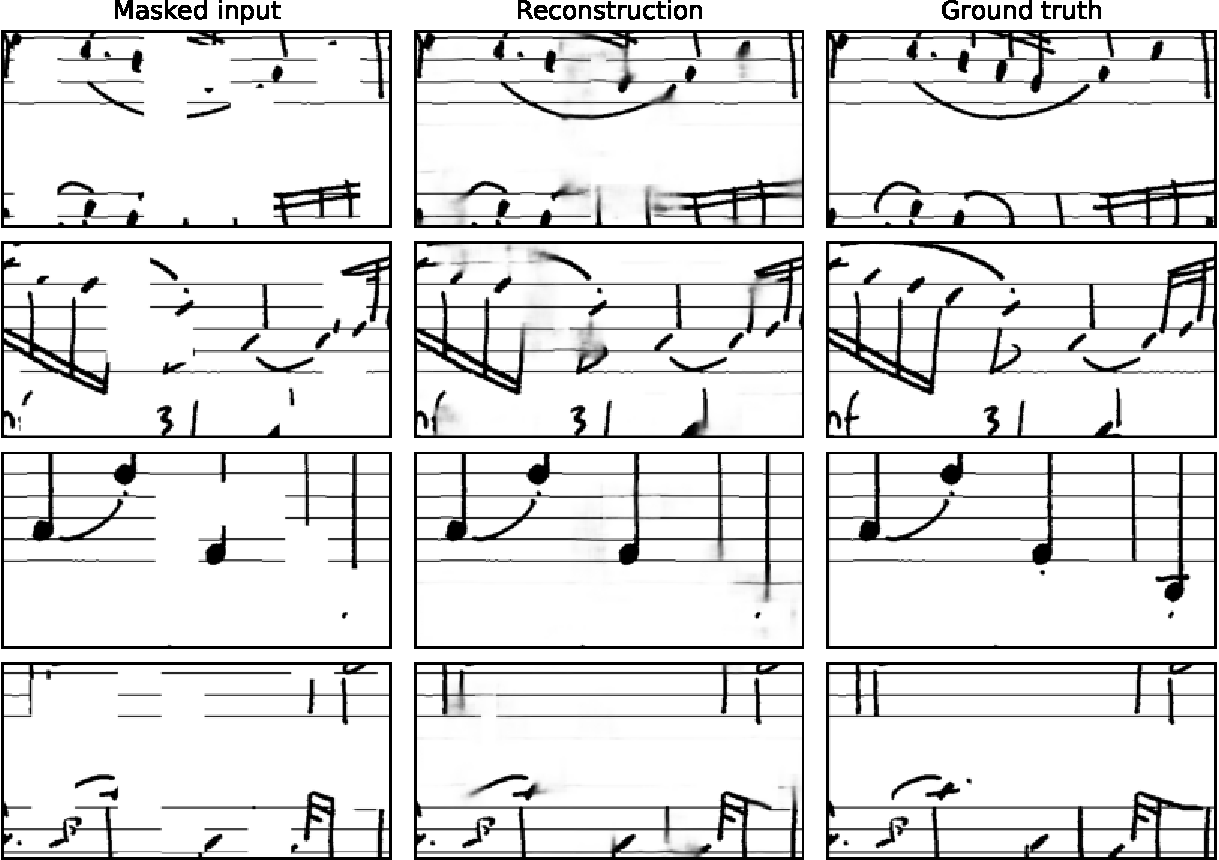
\includegraphics[width=140mm]{../../figures/06-noise/reconstructions.pdf}
    \caption{Our training scheme manages to train a U-Net architecture in an unsupervised manner to produce reconstructions of masked images. Each row is an example of a performed reconstruction (middle), together with the input and expected output. We can see that stafflines are reconstructed very well, whereas more complicated symbols tend to get blurred out.}
    \label{fig:Reconstructions}
\end{figure}

We train the model in the context of three experiments and compare it against a corresponding supervised baseline. The model prediction is evaluated using pixelwise F1 score, as it aggregates both precision and recall into a single number. Performing the evaluation pixelwise lets us compare the model to the baseline with minimal added complexity (e.g.\@ bounding box detection) and thus provide direct feedback on the only property varied -- the amount of unlabeled data.

All three experiments suggest, that training a U-Net in this semi-supervised scheme acts as regularization and helps stabilize the training. Unfortunately, we did not manage to surpass the supervised baseline, we only got the same performance. We belive that training the reconstruction with pixelwise binary cross entropy loss function causes the model to produce fuzzy reconstructions and to learn representations that are not useful for improving segmentation performance. This may be because there are many possible reconstructions of a masked area, and the model learns to reconstruct their fuzzy average, instead of picking one and making a good-looking reconstruction. We belive that adding a smarter loss function, such as a discriminator network, could lead to improvements. We plan to explore this idea in a future work.

% TODO: emphasize thesis contributions as a listing and add experimentation and exploration to it

% TODO: add chapter listing with short descriptions

% TODO: crop away horizontal whitespace from images that should match the pagewidth

Code for the model and all experiments is available in a GitHub repository at \url{https://github.com/Jirka-Mayer/MasterThesis}.

\chapter{Related Work}
\label{chap:RelatedWork}

\section{The U-Net architecture}

The article \emph{U-Net: Convolutional Networks for Biomedical Image Segmentation} (\cite{UNet}) introduces a fully-convolutional neural network, that is surprisingly good at performing image segmentation. The article uses this architecture for semantic segmentation and instance segmentation of various biomedical images.

\begin{figure}[ht]
    \centering
    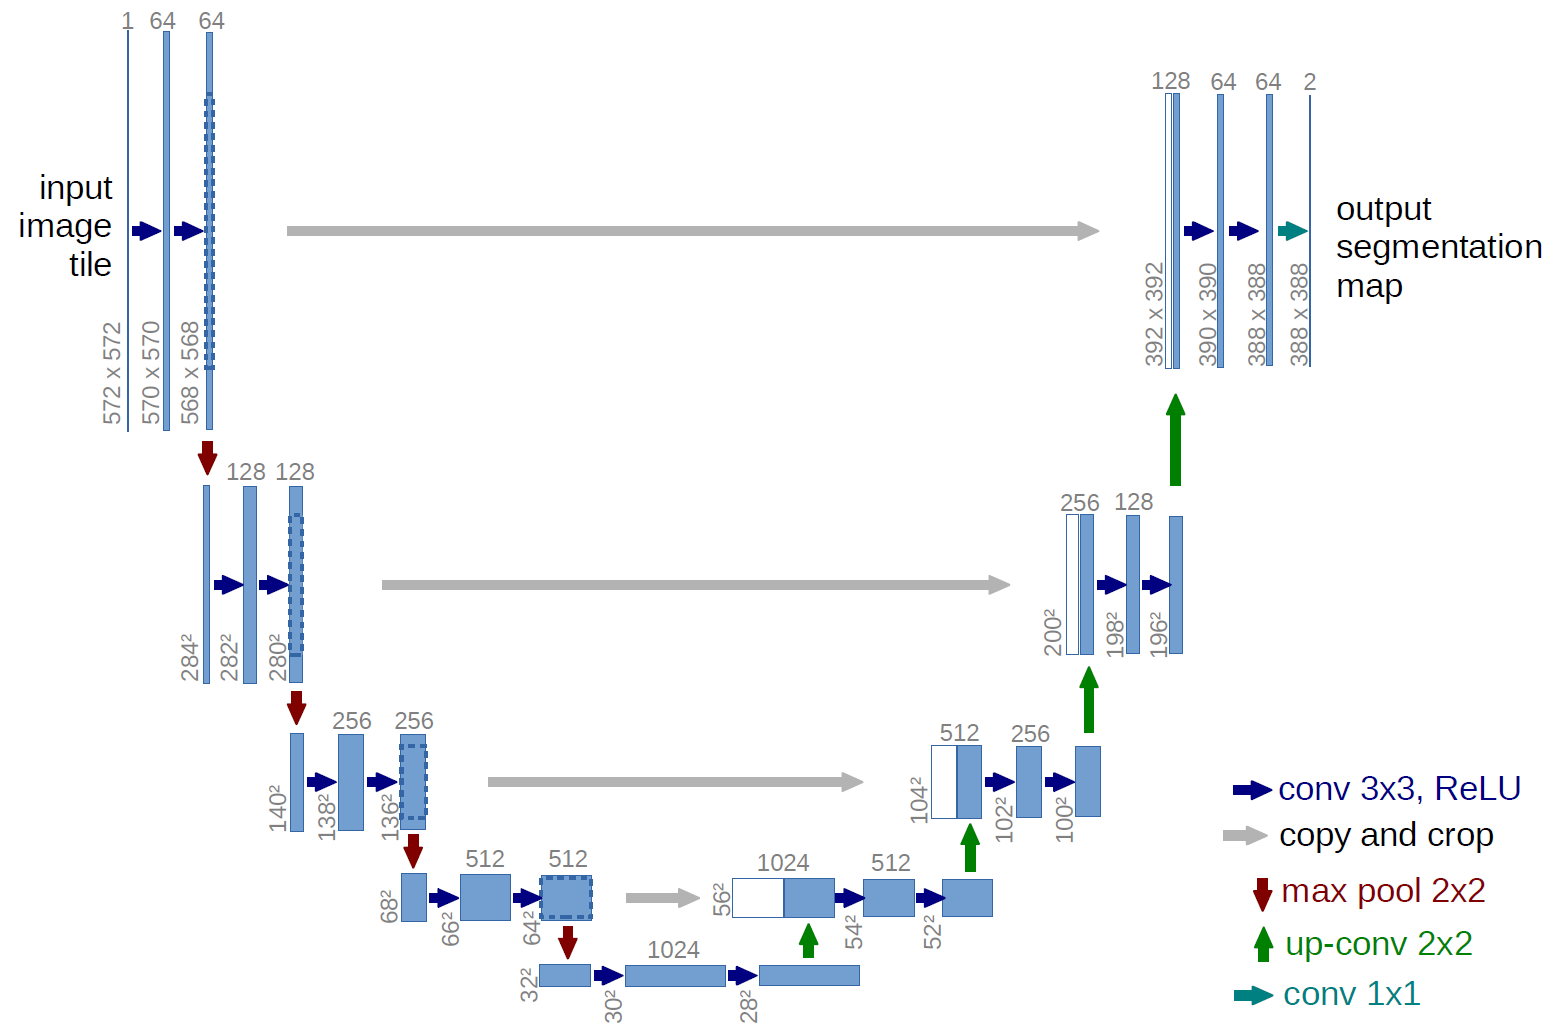
\includegraphics[width=145mm]{../img/u-net-architecture.png}
    \caption{The U-Net architecture with a contracting path and an expansive path. The image is taken from \cite{UNet}.}
    \label{fig:UNetArchitecture}
\end{figure}

The authors describe the left part of the network as the contracting path. It follows the typical structure of a convolutional network. The right part is called the expansive path. It is built as an inverse to the contractive part. The combination of contraction and expansion causes the network to first gather context information around each point of the image and then spread it back out to inform the segmentation process. The two halves are connected using skip-connections, so that the expansive path also has accurate local information available. Since the architecture resembles an autoencoder, we refer to the two halves of the network as an encoder and a decoder. One additional advantage of this architecture is its speed of both inference and training.


\section{Music object detection}

A variation of the U-Net architecture has been first utilized in the context of music recognition in the article \emph{On the Potential of Fully Convolutional Neural Networks for Musical Symbol Detection} (\cite{DorferEtAl}). Authors used it for notehead detection, as a continuation of their previous research into convolutional neural networks for music symbol detection. They managed to outperform other approaches with a much simpler system and faster inference time.

\begin{figure}[ht]
    \centering
    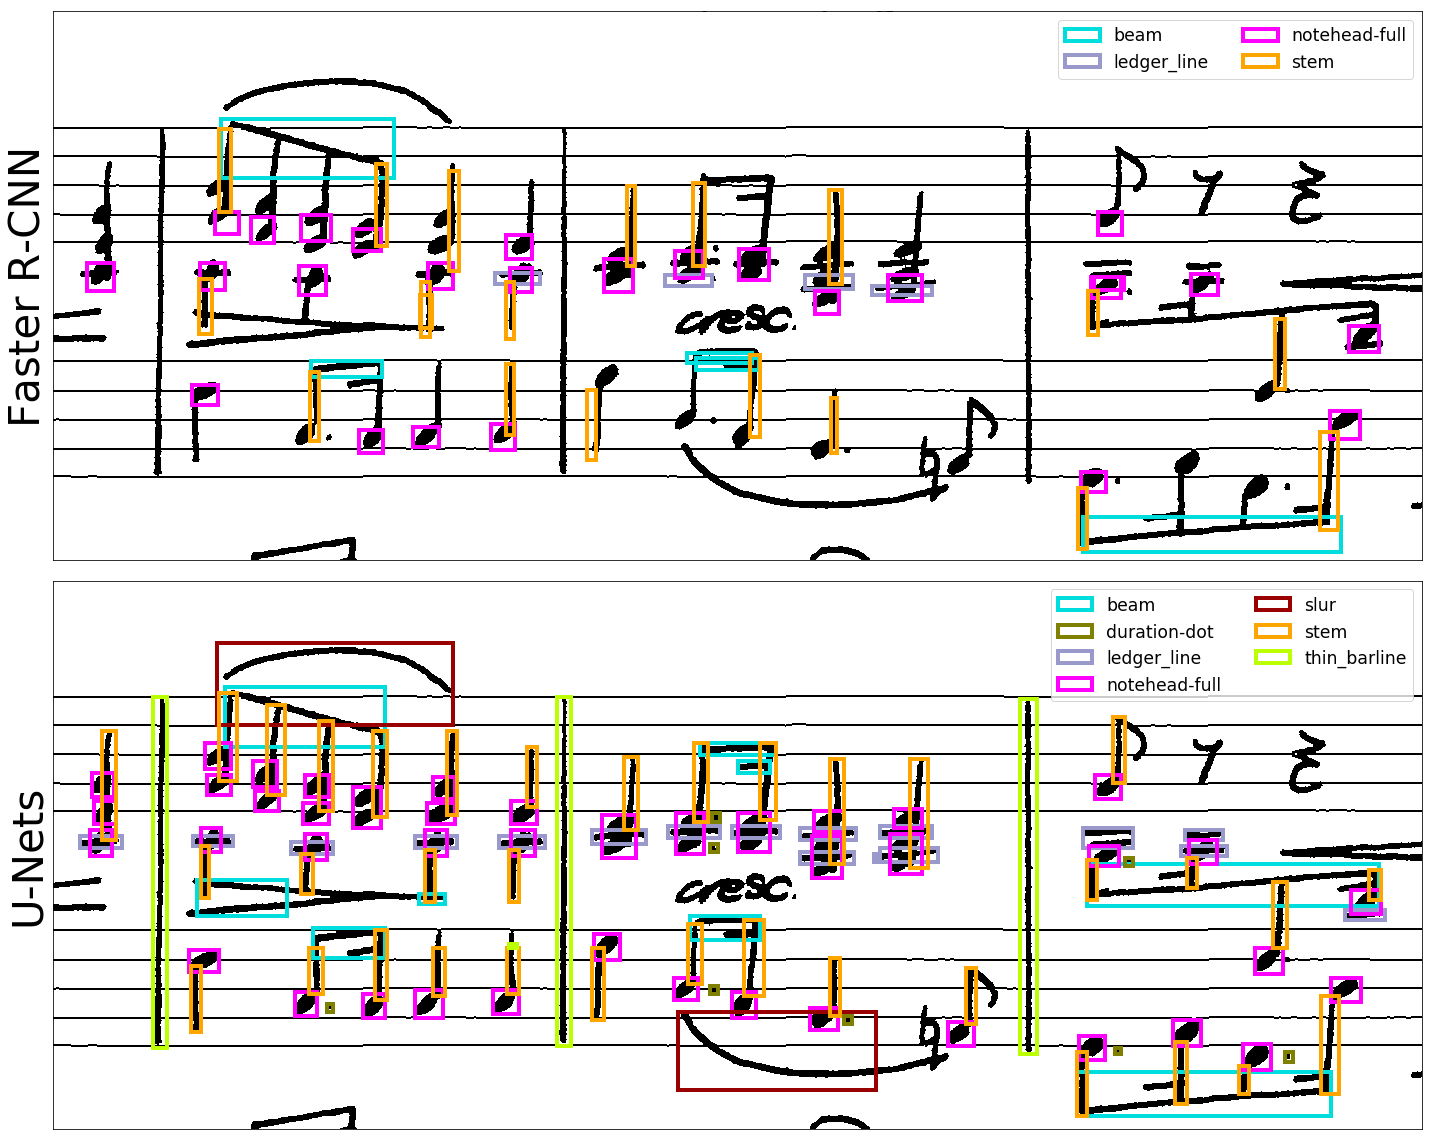
\includegraphics[width=145mm]{../img/muscima-detection-comparison.png}
    \caption{Comparison of the R-CNN and the U-Net architecture for object detection on the MUSCIMA++ dataset. The RetinaNet signle-shot detection is very poor, so the image is omitted to save space. The original image with additional images showing other datasets can be found in (\cite{PachaBaseline}).}
    \label{fig:MuscimaDetectionComparison}
\end{figure}

Both authors then refined the approach in the article \emph{Towards Full-Pipeline Handwritten OMR with Musical Symbol Detection by U-Nets} (\cite{HajicEtAl}). The architecture was extended to perform multi-class segmentation in one pass and domain-specific tricks have been added to increase performance on some symbols. A notation assembly system was designed using decision trees and a complete pipeline with MIDI output was constructed and evaluated.

In the same year, a comparison of object detection architectures for musical symbols was published: \emph{A Baseline for General Music Object Detection with Deep Learning} (\cite{PachaBaseline}). The authors trained three object detection architectures, namely Faster R-CNN, RetinaNet, and U-Net. Their evaluation was performed using three datasets with object detection ground truth, and varied appearance and content. These were the Capitan dataset (mensural notation), the DeepScores dataset (digitally printed modern notation), and the MUSCIMA++ dataset (handwritten modern notation). The article establishes baseline results in different areas of music recognition, but most importantly, identifies the U-Net architecture as the best known architecture for object detection.


\section{Generative semi-supervised learning}

TODO: All the unsupervised, semi-supervised, clustering and disentagnling features of adversarial autoencoders (\cite{AdversarialAutoencoders}). Pioneered by smisup VAE (\cite{KingmaSslVae}).

% adversarial autoencoders
% which has been pioneered by M1+M2 VAE

\chapter{Current State of OMR}
\label{chap:CurrentStateOfOMR}

\chapter{Semi-supervised Learning}
\label{chap:SemisupervisedLearning}

This chapter provides an overview of semi-supervised learning (SSL). The following text draws information predominantly from the article \emph{An Overview of Deep Semi-Supervised Learning} (\cite{SemisupervisedOverview}) and from the book \emph{Semi-supervised learning} (\cite{SslBook}).

In deep learning, the goal typically is to learn some function $f: X \rightarrow Y$ by training a neural network on pairs of data points $(x, y)$. Deep neural networks have large number of trainable parameters, which require adequately large training datasets. Not having enough training data causes the model to overfit and then be unable to generalize to unseen data. Producing training datasets requires a lot of manual labour. Obtaining input data from the domain $X$ is typically easy, the difficult task is assigning correct outputs from $Y$ (called labeling). For this reason, many niche domain problems (e.g. handwritten music recognition or cuneiform recognition) lack sufficiently large labeled datasets for training deep learning models (\cite{MuscimaPP}, \cite{Cuneiforms}). These domains, however, have a relative abundance of unlabeled data.

Semi-supervised learning is a set of methods that aim to utilize this unlabeled data in addition to the available labeled data. The goal of these methods is to produce models that perform better, than models trained on the labeled data alone. The field of SSL has emerged in 1970s and has since accumulated a number of techniques. This thesis focuses on a subset of these techniques, that are based on generative models. However, this chapter provides a short overview of other available techniques as well.

\begin{figure}[p]
    \centering
    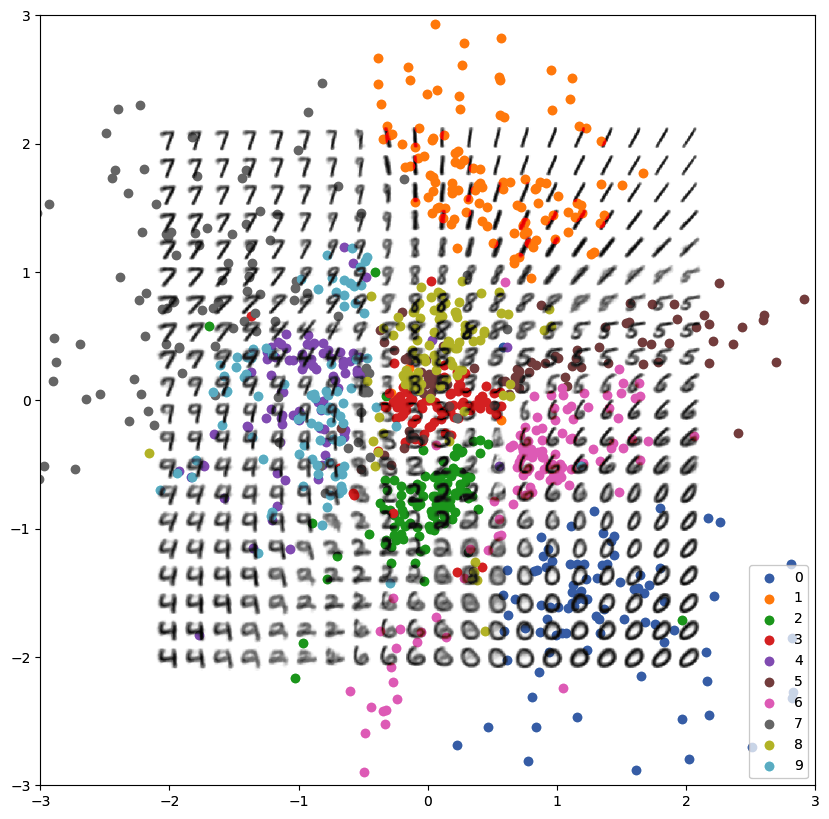
\includegraphics[width=140mm]{../img/mnist-manifold.png}
    \caption{Variational autoencoder learns to project 784-dimensional space of MNIST images down to only 2 dimensional space. We can see clusters of individual classes, forming high-density regions and being separated by low-density regions.}
    \label{fig:MnistManifold}
\end{figure}

\begin{figure}[p]
    \centering
    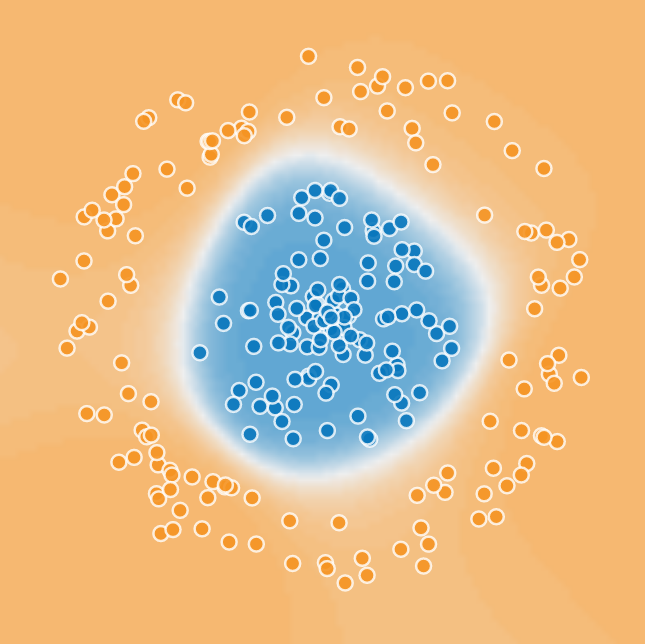
\includegraphics[width=50mm]{../img/decision-boundary.png}
    \caption{Visualization of a classification task, with the decision boundary visible in between the two classes (the while region).}
    \label{fig:DecisionBoundary}
\end{figure}

\qquad

The following text uses a couple of terms, that should be explained first. We will do that on an example:

The figure \ref{fig:MnistManifold} shows the latent space of a variational autoencoder trained on the MNIST dataset (\cite{VariationalAutoencoder}, \cite{Mnist}). This dataset contains grayscale images of handwritten digits, 28x28 pixels in size. In machine learning, the \emph{manifold hypothesis} states, that \emph{real-world high-dimensional datasets lie along low-dimensional manifolds inside that high-dimensional space}. The space of all 28x28 images is such a \textbf{high-dimensional space} (784 dimensions). Manifold, mathematically speaking, is a continuous, locally-eucleidian space (e.g. a plane, sphere, 3D space, Möbius strip). The latent space of the autoencoder is a 2D plane (as seen in the figure \ref{fig:MnistManifold}) and it is the stated \textbf{low-dimensional manifold} containing all the data. Our data points lie on this manifold, the model has only learned, how is this 2D manifold embeded in the 784-dimensional space. (Note that it is not the only manifold the data lies on, this is just the one the neural network discovered during training.)

Data points are not evenly scattered throughout the high-dimensional space. They are coalesced into groups called \textbf{clusters}. Points within these clsuters are located relatively close to each other and usually share the same class. This is an equivalent statement to saying that all digits 7 look alike. These clusters are clearly visible in the latent space (fig. \ref{fig:MnistManifold}), where they form very distinct blobs. The space, where clusters sit, is refered to as \textbf{high-density regions} -- many items from the dataset are located here. Conversely, the space between clusters, where almost no data points are present, is refered to as \textbf{low-density regions}.

A classification task learns a function that assigns a label to each point of the input space. This label is discrete. We can color the input space according to the assigned label and that would produce regions, where all points have the same label. The place where these regions meet is called the \textbf{decision boundary}. A decision boundary can be seen in figure \ref{fig:DecisionBoundary}. In a well-trained classifier for a well-defined classification problem, this decision boundary should lie in the described low-density regions.


\section{Assumptions}
\label{sec:SslAssumptions}

Before we start using semi-supervised methods, we should first understand assumptions that underpin them. These assumptions are mostly intuitive and are satisfied in almost all real-world problems, however stating them explicitly yields better understanding of these methods.

\begin{itemize}
    \item \textbf{The Smoothness Assumption.} \emph{If two points $x_1$, $x_2$ reside in a high-density region and are close together, then their corresponding outputs $y_1$, $y_2$ should also be close together.} For example, if we have a picture of digit 7, then small variations in its shape and color should still be interpreted as digit 7. The opposite statement also holds; if the two input points are separated by a low-density region, the outputs must be distant from each other. This assumption is primarily helpful in a classification task, not so much in a regression task.
    \item  \textbf{The Cluster Assumption.} \emph{If points are in the same cluster, they are likely to be of the same class.} This assumption connects the classification task to the smoothness assumption. It indirectly states, that the decision boundary is located in low-density regions, because otherwise it would cut a cluster in half, causing close points to fall to different classes (which is a violation of the assumption). This assumption can be used as a motivation for methods that push the decision boundary away from data points, into the low-density regions.
    \item \textbf{The Manifold Assumption.} \emph{The (high-dimensional) data lie (roughly) on a low-dimensional manifold.} The problem with high-dimensional data is that as the number of dimensions increases, the volume of the space grows exponentially. This means that most of the space is not covered by any data points in our dataset and that makes it difficult to learn to classify. This assumption states, that our data points actually lie on a small subspace (manifold) of the entire space and that a projection can be learned, that maps this manifold onto a low-dimensional space. Learning the classification task for this low-dimensional space should be much easier.
\end{itemize}


\section{Methods}
\label{sec:SslMethods}

The following section lists major SSL methods. These methods are often directly based on previously stated assumptions and are not mutually exclusive, in fact most of them can be used simultanously as so-called holistic methods. These are, however, not covered in this chapter.


\subsection{Consistency Regularization}

The core idea of this method is that a small neighborhood of each datapoint should have the same label as that datapoint. This idea follows directly from the cluster assumption. In this method, we train the model to minimze distance between a known datapoint $x$ and a perturbed datapoint $\hat{x}$. This training is performed in addition to the usual supervised training. This method does not rely on the corresponding label $y$, instead it trains to minimize the distance between $f(x)$ and $f(\hat{x})$. This lets us utilize all unlabeled data points as well.

The method can be seen as an extension of supervised learning. In supervised learning, we train on individual points and learn the overall shape from them. Here, we train on small neighbourhoods, which makes sure the decision boundary will not come close to any individual datapoint. Further utilization of unlabeled data points in the proximity of labeled data points should force the decision boundary even further away, into low-density regions.


\subsection{Proxy-label Methods}

This is a set of methods, that train a supervised model on the labeled data and then use it to label portion of the unlabeled data. These methods are also called \emph{bootstrapping}. To distinguish these later-added labels, they are called \emph{pseudo-labels}.

One of these methods is \emph{self-training}. In self-training, labeled data is used to train a supervised classification model. This model is then used to classify all unlabeled data points and since its output is a softmax layer, we can not only pick the most likely class, but also measure the confidence in that class. We define a threshold $\tau$ and only assign pseudo-labels to data points above this threshold. This process can be repeated, until a stopping condition is met (e.g. there are no more unlabeled points with confidence above $\tau$). The main problem of this method is the inability to correct mistakes made during the labeling step.

\emph{Pseudo-labeling} is a similar method, where the unlabeled data points are also assigned pseudo-labels. In this case, these pseudo-labels are treated as trainable parameters, similar to model parameters, and are optimized together with the model during training. The difficult part is designing a good loss function for pseudo-labels, because applying this method naively causes the pseudo-labels to overfit, due to so-called confirmation bias.


\subsection{Graph-based Methods}

These methods frame the problem in the language of graphs. Data points are represented as vertices of a graph and weighted edges are present between pairs of vertices, where the weight corresponds to some similarity between the two points. The labeling task can be viewed as a propagation of information along edges of the graph.

This propagation resembles proxy-label methods, however due to the graph framing, we can consider things like vertex neighbourhood and its impact on the examined node, or we can leverage algebraic structures like adjacency matrix.

A different set of graph methods aims to learn data point embeddings, which preserve the structure of the input graph. The goal is to represent each vertex (data point) as a low-dimensional vector, where a simple similarity function (e.g. inner product) can be used. This again resembles deep learning techniques, such as autoencoding (see figure \ref{fig:MnistManifold}), however here, methods derived from graph theory are used to produce these embeddings (e.g. Laplacian Eigenmaps or Locally Linear Embeddings).


\subsection{Entropy Minimization}
\label{sec:EntropyMinimization}

Consistency regularization methods attempt to push the decision boundary away from clusters and into the low-density regions by stabilizing the model output in a neighborhood around each data point. Entropy minimization is a different technique that attempts to do the same thing. In entropy minimization, we penalize the model for being unsure about its predictions. Low-confidence predictions are predictions with more than one class having non-zero probability. Such probability distributions have higher entropy than one-hot distributions. By adding a loss term that minimizes entropy of predictions during training, we can make areas around datapoints more stable. This method can not, however, be used alone for high-capacity models (deep neural networks), as it causes the training to overfit. Instead, it may be used as a supplementing technique to another SSL technique.


\section{Generative Methods}
\label{sec:GenerativeSslMethods}

Generative semi-supervised learning leverages generative models for the classification task. A generative model learns to describe the distribution of data $p(x)$. The assumption here is that this understanding helps the model with the classification task $p(y|x)$. Generative SSL can be viewed either as an extension of supervised learning (classification with the addition of $p(x)$ modeling), or as an extension of unsupervised learning (modeling, extended by label information).


\subsection{Variational Autoencoders}

A variational autoencoder (VAE) (\cite{VariationalAutoencoder}) is a model that attempts to learn a mapping between the input space and a smaller latent space. The latent space is also required to roughly follow a unit gaussian distribution, which causes the space to be filled and smooth, such that sampling any point of this space yields a reasonable corresponding data point. Moreover, the model architecture forces clusters of similar data points to occupy roughly gaussian-shaped regions in the latent space. A visualization of this latent space can be seen in figure \ref{fig:MnistManifold}. The variational autoencoder consists of an encoder and a decoder. The encoder learns the mapping from the input space to the latent space and the decoder learns the inverse mapping. The decoder is then considered as the generative model, as it can generate a reasonable data point for an arbitrary latent space point. Input data points are typically denoted $x$ and the latent vectors are denoted $z$.

\cite{KingmaSslVae} used variational autoencoders in a semi-supervised setting. They propose three ways of extending VAEs:

\paragraph*{M1 Model}
We start by pre-training an unsupervised VAE model using all available labeled and unlabeled samples. The goal is to learn a low-dimensional latent space and then transform all data points to this space (create embeddings). After this, we train a supervised classifier on these embeddings using only the labeled portion of the data. This setup leverages the manifold assumption and the assumption that learning classification in a low-dimensional space is easier than in a high-dimensional space. Also, since the variational autoencoder forces the creation of gaussian-shaped clusters in the latent space, the classifier has an easier job separating these clusters.

\paragraph*{M2 Model}
In the previous setup, we ignored labels $y$ when training the autoencoder. Here, we extend the latent vector $z$ by an additional vector $y$. This vector will be set to the label, if the label is known and will be left unconstrained for unlabeled data. We can view this as splitting the original latent vector $z$ into two parts, one being left free to be trained as usual, and the second (categorical) part being sometimes trained to match the label $y$ of the learned datapoint $x$. If the label is not known, this part is trained in the unsupervised mode only, like the original latent variable $z$. When the training finishes, the encoder can be immediately used as a classifier, by interpreting the latent vector $y$ as the output label. The two parts of the latent representation ($z$ and $y$) can be interpreted as style and content embddings respectively.

\paragraph*{M1 + M2 Model}
The last setup involves training the model M1 in the unsupervised way and then training the model M2 in semi-sueprvised way on embeddings produced by M1. It can be viewed as the M2 model, utilizing dimensionality reduction by M1. This stacked setup yields the best results.


\subsection{Adversarial Autoencoders}

A newer article by \cite{AdversarialAutoencoders} introduces an architecture, called an Adversarial Autoencoder (AAE). The architecture is in many ways similar to the variational autoencoder, but it differs in the way it regularizes its latent space. Whereas a VAE uses KL-divergence loss to force the latent space into a gaussian distribution, an AAE uses a discriminator network (inspired by generative adversarial networks). This architecture can be used and extended in similar ways to the M1 and M2 models and yields even better results for tasks, such as semi-supervised classification, unsupervised clustering and style-content disentangling.


\subsection{Generative Adversarial Networks}

Generative adversarial network (GAN) is a generative architecture consisting of two parts: a generator and a discriminator. They are trained together in an alternating fashion, where the generator is trained to produce realistic-looking data (to fool the discriminator) and the discriminator is trained to distinguish this generated data from the real-world data. The tension between these two models causes both of them to get increasingly better and the generator ends up producing well-looking synthetic samples. Input to the generator is a latent vector $z$, drawn from a prior distribution (e.g. a gaussian). The generator uses this vector as a seed for the generation. The discriminator outputs a single value, interpreted as the probability of the shown sample being real or generated.

\paragraph*{CatGAN}
Categorical generative adversarial networks (CatGAN) replace the discriminator with a classifier. The output of this classifier is a softmax layer with C neurons. The discriminative task is transformed onto the classifier by considering its certainty of prediction. In the section on entropy minimization (\ref{sec:EntropyMinimization}), we described how certainty of prediction is related to entropy of the predicted distribution, and also how the entropy can be minimized (or maximized) to force the model to be certain (uncertain). In the unsupervised mode, the classifier is trained to output one (any) of the classes for real data points with maximum certainty -- to recognize real samples. The generator is then trained to confuse the classifier to produce uncertain predictions (uniform distribution).

In SSL, the classifier is trained to produce confident predictions of any class for unlabeled data and confident predictions of known class for labeled data. The supervised loss is a categorical cross-entropy (like in a typical classification setup) and the unsupervised loss is an entropy minimization loss (to force confident predictions of any class).

\paragraph*{DCGAN, SGAN}
Deep Convolutional GANs attempt to learn intermediate representations by training convolutional GANs on unlabeled data. Parts of the generator and discriminator are then re-used as feature extractors for supervised classification task. Semi-supervised GANs (SGAN) address and fix issues with DCGAN, such as the fact that the classifier is trained after the GAN has finished training. SGAN is able to train the generator and classifier simultaneously, substantially improving classification performance.

\paragraph*{BiGAN}
In a typical GAN, the latent variable $z$ is only used as a seed for the generator and the generator acts as function $G: Z \rightarrow X$. In a variational autoencoder, there exists a full bijection between spaces $X$ and $Z$. BiGANs extend the basic GAN framework by adding an encoder, that acts as a mapping $E: X \rightarrow Z$. This gives us access to the latent vector $z$ of an existing real-world sample $x$. The discriminator is extended to have access to both the data points and the latent points, and so it discriminates between pairs of $(x, E(x))$ and $(G(z), z)$. BiGAN therefore serves a similar role to a variational autoencoder and can be extended for use in semi-supervised learning.


\section{Related Methods}
\label{sec:RelatedSslMethods}

\paragraph*{Transfer Learning} In transfer learning, the goal is to utilize the knowledge about one problem to solve another different but related problem. For example, utilizing layers of an already trained network (e.g. an autoencoder) as feature extractors for a different task (e.g. classification) is an example of transfer learning.

\paragraph*{Domain Adaptation} In the previous example of transfer learning, the two tasks have different feature space. Domain adaptation is a subset of transfer learning where both tasks have the same feature space, but different data distribution. For example, training a classifier of handwritten digits on augmented printed digits (handwritten and printed digit images are both images, just with different distributions). Semi-supervised learning differs from domain adaptation in that both problems have the same data distribution (the training and test data come from the same process).

\paragraph*{Muti-task Learning} Multi-task learning is the process of training one model to solve two different tasks simultaneously. By having one model learn both tasks, the model can share intermediate representations for both of them, achieving better performance, than by having a dedicated model for each task.

\chapter{Experiments and Results}
\label{chap:ExperimentsAndResults}

TODO: quick chapter overview

\begin{code}
$ python3 main.py unet train --val_pages 123 ...
\end{code}


\section{Architecture}
\label{sec:Architecture}

In the \emph{generative model} approach to semi-supervised learning, one usually starts with a model that can be trained in the unsupervised manner (either an autoencoder or a generative adversarial network [CITE, CITE]) and then extends it to also perform the supervised task. For example, when starting with an autoencoder, one can use the encoder part as a dimensionality reduction mechanism and then build a supervised classification network that classifies the learned embeddings [CITE].

In our context of music recognition, we are highly motivated to build on top of the U-Net architecture [CITE] (figure \ref{fig:ArchitectureCombined}). It has first been used for biomedical image segmentation, however its superiority for object detection in music recognition has clearly been demonstrated by Pacha et al. [CITE].

The architecture can be viewed as a fully convolutional autoencoder with residual (skip) connections added between the encoder and decoder on every resolution level. The U-Net encoder is a typical fully-convolutional encoder that gradually reduces image dimensions, while increasing the channel count. Such an architecture is able to learn abstract representations of symbols present in the input image. The decoder then tries to go from these abstract representations back to specific ones, while at the same time modifying the reconstruction to fit the learned segmentation task. The core idea behind this architecture is that the decoder can utilize skip connections during upsampling, thereby producing a pixel-perfect segmentation.

\begin{figure}[ht]
    \centering
    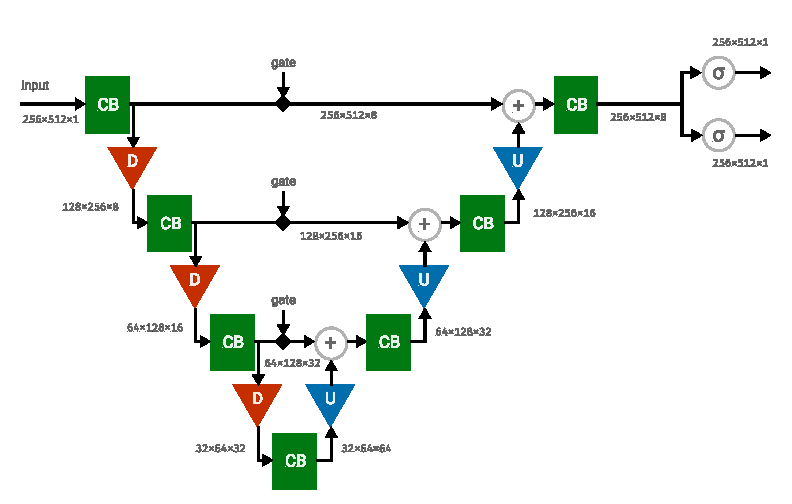
\includegraphics[width=140mm]{../img/architecture-complete.pdf}
    \caption{TODO}
    \label{fig:ArchitectureCombined}
\end{figure}

We choose to share the entire U-Net model for both the supervised and unsupervised tasks. The two tasks are differentiated only at the very last layer. The original U-Net architecture ends with a 1x1 convolution layer with sigmoid activation. It can be viewed as a pixelwise softmax for two output classes of a typical classification model. We decided to fork the architecture here, having one sigmoid convolution for the supervised segmentation task and one for the unsupervised reconstruction task.

The supervised task can be trained in almost the same way as the the original U-Net archtiecture:

\begin{itemize}
    \item A batch $(x, y)$ of input images and expected segmentation masks is taken from the dataset.
    \item Input images $x$ are fed through the model, producing a prediction for the segmentation mask $\hat{y}$ and for the reconstructed image $\hat{x}$.
    \item A loss function is used, computing the distance between $y$ and $\hat{y}$ and generating gradients for the network.
    \item Reconstruction output $\hat{x}$ is ignored and no gradients for the branch are computed.
    \item An optimizer uses computed gradients to update model parameters.
\end{itemize}

The unsupervised task could be trained in the same way, using the other output branch of the model. This would work for a typical autoencoder, but since the U-Net architecture contains skip connections, the model could learn an identity function without using any of the abstraction-learning layers. The goal of unsupervised learning is learning these abstract features, so this training scheme is infeasible in our context.

We propose two ways of overcoming this challenge:

\begin{itemize}
    \item gated skip connections
    \item denoising
\end{itemize}

One option is to disable skip connections during reconstruction training and keep them enabled during segmentation training. This should force the model to learn abstract features during reconstruction, while also being able to utilize skip connections during segmentation. This scheme performs much better than a typical autoencoder without any skip connections, but is still outperformed by the next proposed scheme (see detailed comparison in section \ref{sec:SkipConnections}).

The second option is add some noise to the input image during reconstruction training. The model would learn to not only reconstruct the input image, but also to remove the added noise. We took inspiration from denoising autoencoders [CITE AUTOENCODERS]. The difficult part is designing the noise function such that it would cause the model to learn abstract representaions (see section \ref{sec:NoiseGeneration}).

We consider the described scheme for unsupervised U-Net training to be the main contribution of this thesis. The proposed experiments try to assess the viability of the scheme in the context of semi-supervised learning.

Both the segmentation and reconstruction tasks are trained jointly on composite batches and a single composite loss function. A single optimizer step is used to update model parameters for both tasks. The process is described in detail in section \ref{sec:Training}.

% - Denoising U-Net
%     - what input/output combinations we will use
% - multiclass options
%     - output channels
%     - multiple decoders
%     - seems not to improve, rather worsen if used incorrectly \[hajic\]
% - describe the architecture (as seen in the image)
%     - upsampling block details

\begin{figure}[p]
    \centering
    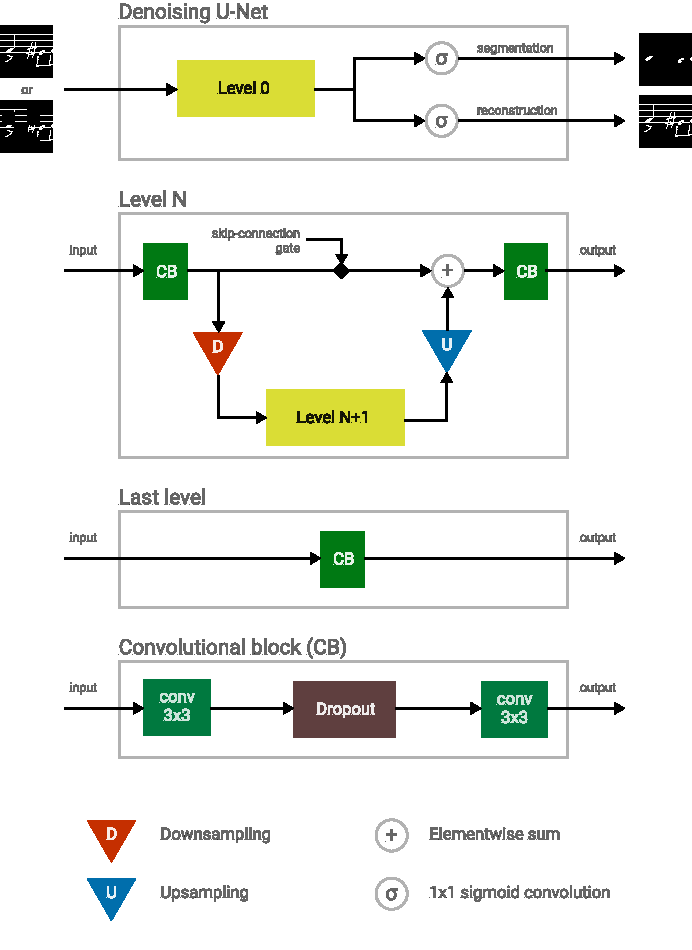
\includegraphics[width=140mm]{../img/architecture-pieces.pdf}
    \caption{TODO}
    \label{fig:ArchitecturePieces}
\end{figure}


\section{Datasets}
\label{sec:Datasets}

% - MUSCIMA++
% - DeepScores
%     - https://arxiv.org/pdf/1804.00525.pdf
%     - v2: https://ieeexplore.ieee.org/document/9412290/
% - solving resolution problems
% - solving stability (dataset seed) when increasing unsupervised ratio (fixing sup split, growing unsup split)


\section{Noise Generation}
\label{sec:NoiseGeneration}

% - why large noise -> to learn representaions?
% - mention cuneiform article from ICDAR - GAN reconstruction
% - noise generation and parameters


\section{Training}
\label{sec:Training}

% - composite batches
% - training both simultaneously
% - loss function
% - pick the model with the lowest validation loss over a training session


\section{Evaluation Metrics}
\label{sec:EvaluationMetrics}

% - F1 score
% - pixelwise vs. object detection
%     - reference other works and their approach
%     - pixelwise isn't directly telling about object detection performance
% - thresholding due to varying image resolution

% - object detection metrics overview:
%     https://towardsdatascience.com/evaluating-performance-of-an-object-detection-model-137a349c517b


\section{Semi-supervised Improvements}
\label{sec:SemisupervisedImprovements}

The main hypothesis this work is attempting to validate is that adding unlabelled data to the training process helps. We primarily want to improve model accuracy, but as we will see, this is not what our experiments suggest. They do, however, show improvements in other areas, such as training stability and reduced overfitting (section \ref{sec:UtilizingCvcMuscima}).

In the first experiment, we test how various labeled to unlabeled data ratios affect the training process. The experiment uses the MUSCIMA++ dataset [CITE]:

\begin{itemize}
    \item 10 pages act as the labeled set.
    \item 0, 5, 10 and 50 pages act as the unlabeled set.
    \item 10 pages act as the validation set.
    \item All of these pages come from the writer-independent train set of MUSCIMA++ and are chosen in a writer-independent manner (all the splits contain pages by different writers).
\end{itemize}

The learned task is notehead segmentation (both full and empty noteheads). Noteheads are an ideal symbol for this kind of measurement. Firstly, they are very abundant. Each page of the dataset contains many instances of them and they are evenly scattered over the whole page. If we were to instead detect more rare symbols (such as clefs or rests), it could skew the results, making it difficult to separate the effects we want to measure. Handwritten noteheads are also very diverse in style, making them more interesting to learn (compared to, say, stafflines).

All model hyperparameters are set to sensible deafults. The derivation of these values is desribed later in section \ref{sec:UnderstandingHyperparameters}. The model capacity, described by the \emph{inner features} parameter is set to 8, which is useful to know for comparison with the next experiment. The proposed dataset is rather small and so the training is very noisy (figure \ref{fig:ExplorationNoteheadsNoDropout}). To stabilize the trainig we set the dropout parameter to 50\% [CITE DROPOUT].

\begin{figure}[ht]
    \centering
    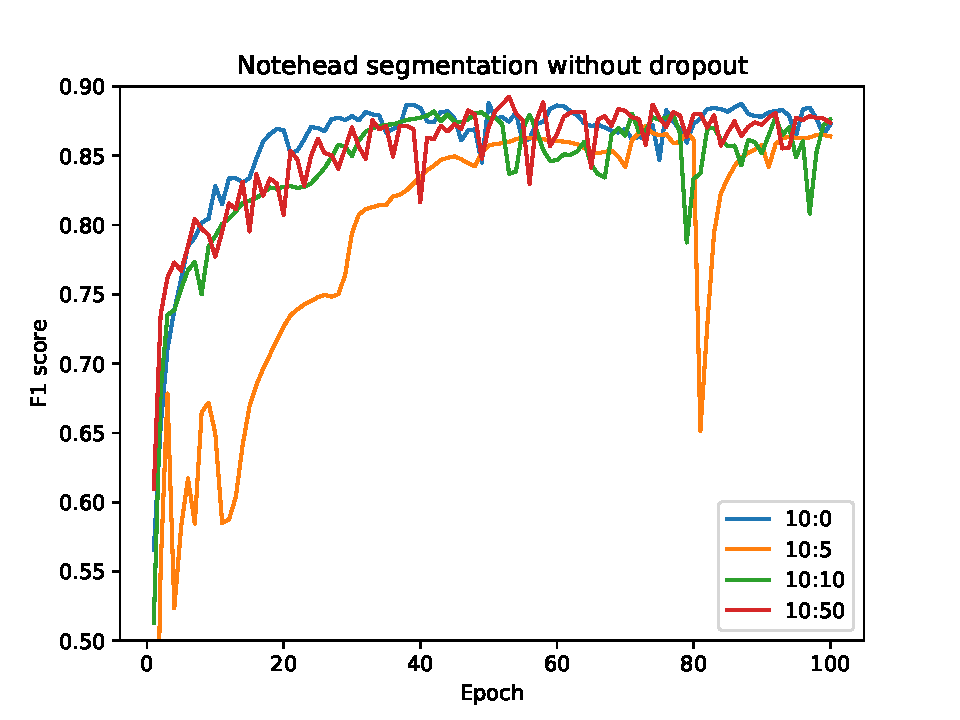
\includegraphics[width=140mm]{../../figures/01-exploration-noteheads/noteheads.pdf}
    \caption{Training on a small dataset without dropout is noisy, see the orange line at the beginning and the green line at the end.}
    \label{fig:ExplorationNoteheadsNoDropout}
\end{figure}

We expect that as we add more and more unlabeled data, the F1 score should reach higher and higher. Or at least not get worse. This is not what we see in the figure \ref{fig:ExplorationNoteheads}. The fully supervised model outperforms all the others by a clear margin.

Focusing only on the semi-supervised models, it seems that adding more unsupervised data maybe helps here, although the three lines end up on top of each other at the epoch 200. A better idea is to look at the figure \ref{fig:ExplorationNoteheadsEvaluation}. The chart contains evaluation results on the test set of six runs of each configuration. We can clearly see how the performance rises with more unsupervised data. Unfortunately it does not reach above the fully-supervised results. We unfortunately cannot push the amount of unlabeled data much higher, as it would break our training process (see section \ref{sec:BatchSize}) and it would likely also have diminishing returns. The actual numbers are summarized in table \ref{tab:ExplorationNoteheads}.

The reason for the drop in performance is actually caused by the fact, that the supervised model has to only learn one task -- segmentation. Whereas the semi-supervised one has to also learn the unsupervised reconstruction task. This claim is explored in the next section and is supported by the fact that the performance drop disappears when we increase model capacity.

\begin{figure}[p]
    \centering
    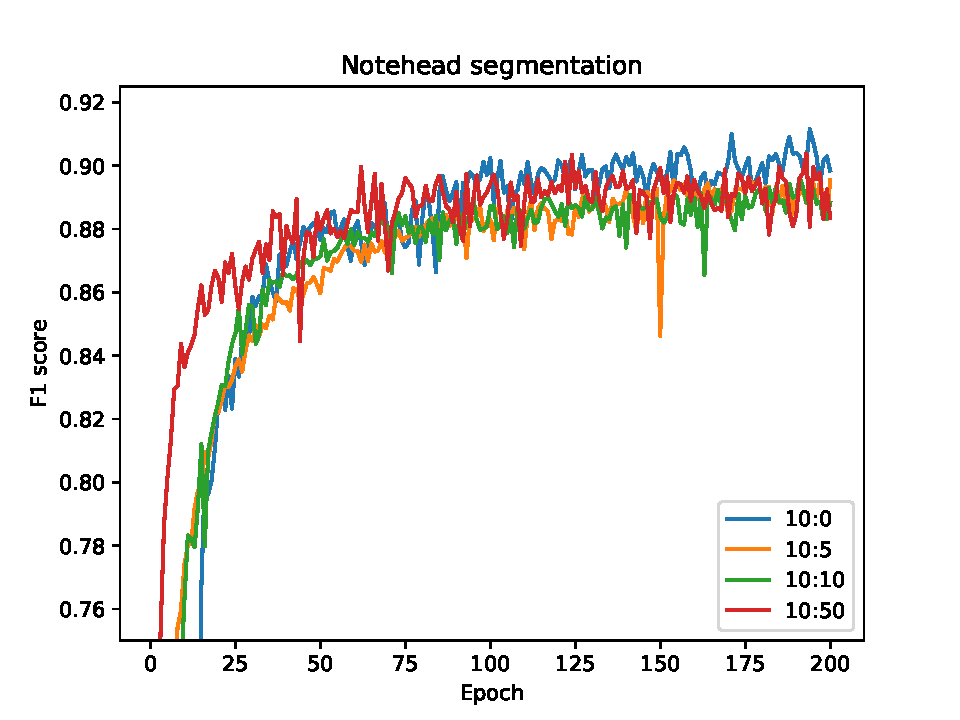
\includegraphics[width=140mm]{../../figures/01-exploration-noteheads/noteheads-dropout.pdf}
    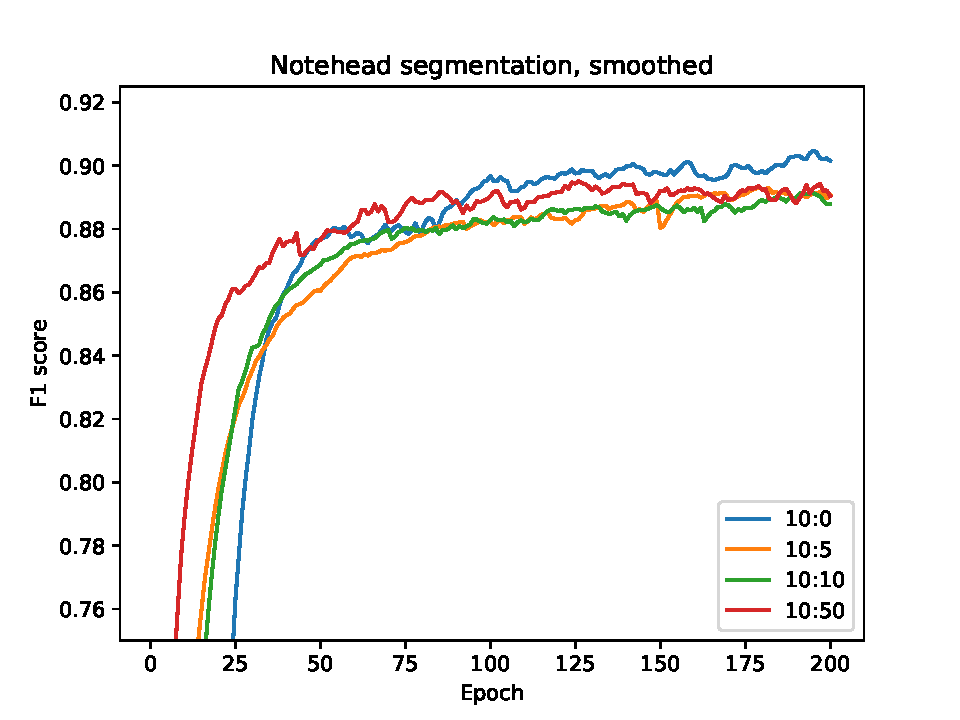
\includegraphics[width=140mm]{../../figures/01-exploration-noteheads/noteheads-dropout-smooth.pdf}
    \caption{Lorem ipsum dolor.}
    \label{fig:ExplorationNoteheads}
\end{figure}

\begin{figure}[ht]
    \centering
    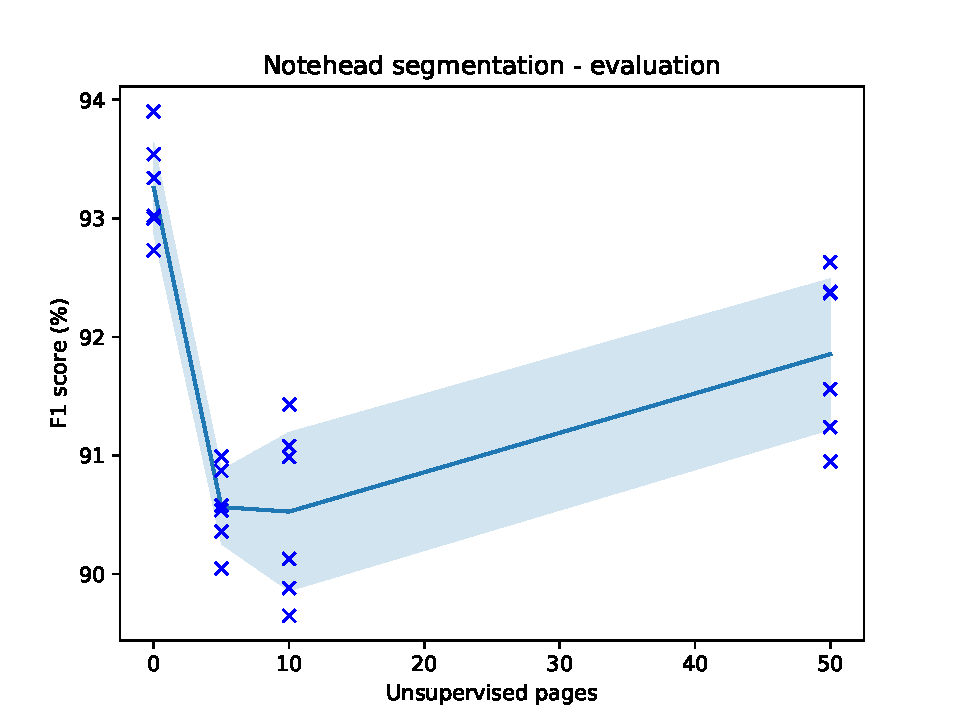
\includegraphics[width=140mm]{../../figures/01-exploration-noteheads/noteheads-evaluation.pdf}
    \caption{Lorem ipsum dolor.}
    \label{fig:ExplorationNoteheadsEvaluation}
\end{figure}

\begin{table}[b!]
    \centering
    \begin{tabular}{l@{\hspace{1.5cm}}D{.}{,}{3.2}D{.}{,}{1.2}D{.}{,}{2.3}}
        \toprule
        & \mc{} & \mc{\textbf{Směrod.}} & \mc{} \\
        \pulrad{\textbf{Efekt}} & \mc{\pulrad{\textbf{Odhad}}} & \mc{\textbf{chyba}$^a$} &
        \mc{\pulrad{\textbf{P-hodnota}}} \\
        \midrule
        Abs. člen     & -10.01 & 1.01 & \mc{---} \\
        Pohlaví (muž) & 9.89   & 5.98 & 0.098 \\
        Výška (cm)    & 0.78   & 0.12 & <0.001 \\
        \bottomrule
    \end{tabular}
    \caption{Lorem ipsum dolor.}
    \label{tab:ExplorationNoteheads}
\end{table}

TODO: show visualization images / qualitative comparison between runs?


\section{Utilizing CVC-MUSCIMA}
\label{sec:UtilizingCvcMuscima}

This experiment attempts to address issues of the previous experiment:

\begin{itemize}
    \item fixed model capacity
    \item small dataset
\end{itemize}

In the chapter \ref{chap:CurrentStateOfOMR} we described the two major datasets for handwritten music recognition: CVC-MUSCIMA [CITE] and MUSCIMA++ [CITE]. The dataset MUSCIMA++ is a highly annotated subset of CVC-MUSCIMA. We can view both datasets together as a single semi-supervised dataset, being 12\% labeled and 88\% unlabeled. To the best of our knowledge, nobody has yet tried to utilize both datasets simulatenously for semantic segmentation.

Hajič jr. and Dorfer [CITE 1, 2] have used the U-Net architecture [CITE] for segmentation and they trained it on the MUSCIMA++ dataset. Their results are very impressive. Being able to further build on their work and improving the model by utilizing unlabeled data from CVC-MUSCIMA would be very helpful for the field of OMR. This experiment attempts to do just that.

We take the whole CVC-MUSCIMA dataset, separate writers from the MUSCIMA++ independent test set, separate 20 pages for validation set and remove other pages from these validation writers. The pages that remain are produced by writers not present in both the test set and the validation set. These remaining pages are partially contained in the MUSCIMA++ dataset (99 pages) and all the other pages are used as unlabeled data (551 pages). Therefore we train on 650 out of 1000 pages of the CVC-MUSCIMA dataset.

Since the dataset is now much larger than in the previous experiment (section \ref{sec:SemisupervisedImprovements}), we no longer need the dropout. In fact, the training is even more stable and individual runs are clearly separated.

This experiment attempts to compare fully-supervised and semi-supervised models, regardless of their capacity. We therefore train various model capacities (the \emph{inner features} model parameter) and then compare the best ones for each setting.

Another difference to the previous experiment is that the ratio of labeled to unlabeled data is fixed and given by dataset sizes. The ratio of 99 to 551 pages corresponds best with the ratio 10:50.

\begin{figure}[p]
    \centering
    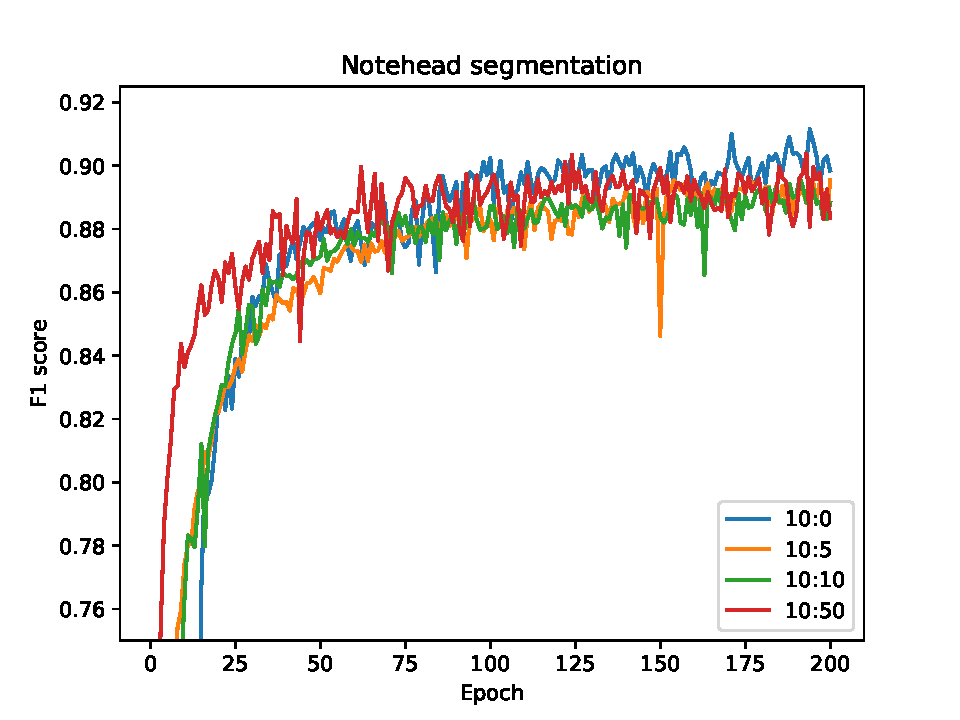
\includegraphics[width=140mm]{../../figures/01-exploration-noteheads/noteheads-dropout.pdf}
    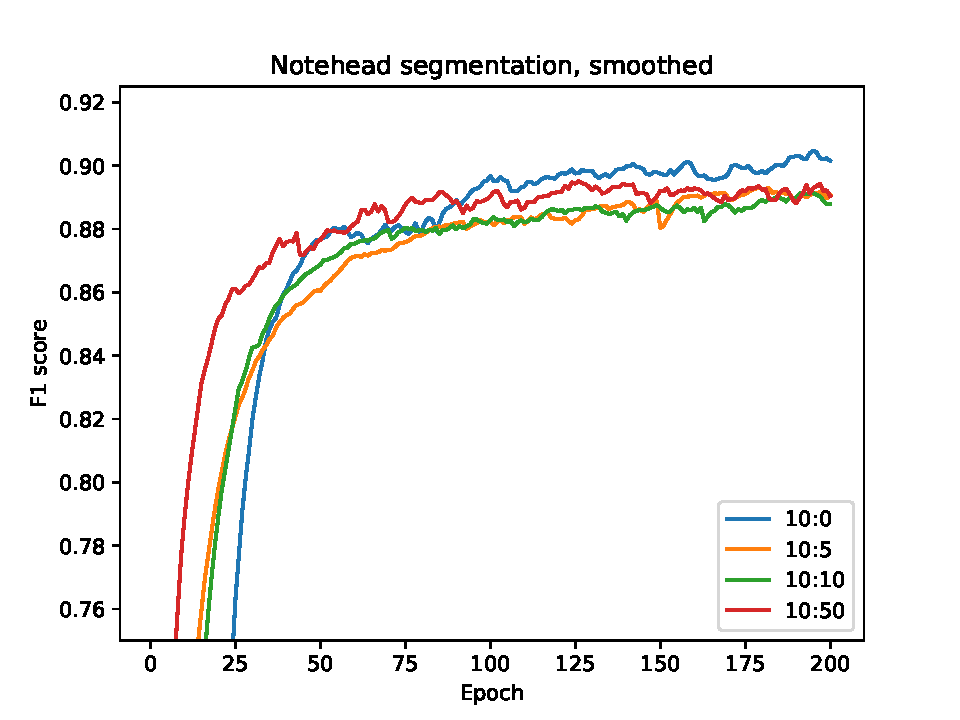
\includegraphics[width=140mm]{../../figures/01-exploration-noteheads/noteheads-dropout-smooth.pdf}
    \caption{Lorem ipsum dolor. TODO: the two improvements charts}
    \label{fig:CvcImprovements}
\end{figure}

The validation dataset F1 score over the course of training can be seen in figure \ref{fig:CvcImprovements}. In these charts we can see:

\begin{itemize}
    \item Models with 1 and 2 \emph{inner features} are clearly underfitting in the supervised mode (compared to other models). When we add the unlabeled data, their perfomance drops significantly, but the training curve gets much smoother.
    \item Models with 4 and 8 \emph{inner features} worsen much less and also get smoother (especially 4 becomes much more stable).
    \item Model 16 no longer worsens, it is able to learn both tasks.
\end{itemize}

Conclusions can be drawn from these observations:

\begin{itemize}
    \item The reconstruction and segmentation tasks clearly compete for model capacity. The performance drop of adding unlabeled data decreases, as the model capacity increases.
    \item The addition of unlabeled data can be used as a regularization technique. This is evident from the fact that training curves get much smoother as we add unlabeled data. A~regularization effect is also described in the corresponding literature [CITE SSL overview].
    \item All models come close to the 96\% line, but never cross it. While the semi-supervised models get as good as the fully-supervised, they never get better. It seems the reconstruction task is not learning any useful representations. [TODO: expand on this further and show reconstruction visualizations - they learn simple shapes, not abstract objects]
\end{itemize}

% TODO: evaluate best models of SUP and SEMISUP, maybe they differ in test score? Probbably not.


\section{Knowledge Transfer}
\label{sec:KnowledgeTransfer}

TODO: knowledge transfer experiment


\section{Understanding Hyperparameters}
\label{sec:UnderstandingHyperparameters}


\subsection{Batch Size}
\label{sec:BatchSize}

In the deep learning field, it is known that having a small batch size makes the training fast and noisy, whereas a large batch size makes it more stable at the cost of being slower [CITE DL BOOK]. Since our model is fully cconvolutional and we train it on image tiles of fixed size, we can consider the size of these tiles to be a parameter similar to batch size. It also regulates the amount of data used for gradient estimation. If the tiles are large enough, we can get away with batch size of 1 (this is what the original U-Net article does [CITE]).

Using such a small batch size is, however, not possible in our case. Our training process expects batches containing both labeled and unlabeled data. Batch size determines the total number of these two kinds of data items in the single composite batch. The ratio of these two item types within the composite batch is dictated by the ratio within the whole dataset. So if our dataset has, for example, 1:5 labeled to unlabeled data, the batch size has to be at least 6. Otherwise we will start getting batches that contain only unlabeled data. This rule isn't as strict, since the model would probably learn both tasks even if half of all batches were missing labeled data, however if the imbalance becomes too severe, the training fails.

TODO: figure with the failing training (bs=2,ratio=1:10)

An example of such a failing training can be seen in figure TODO???. The model learns to perform reconstruction even for the segmentation task. This is understandable, since the two tasks are differentiated only at the last layer (1x1 sigmoid convolution). If all second-to-last layer activations contain image reconstruction data, then any 1x1 convolution combination of them will do as well.

Since all of our experiments have training data ratios between 1:0 and 1:10, we chose to set the batch size parameter to 10.


\subsection{Dropout}
\label{sec:Dropout}

We introduced dropout [CITE] when training on small datasets (section \ref{sec:SemisupervisedImprovements}). The training was so noisy, that it was difficult to infer any measurable differences between runs. Therefore we used dropout as a mean to stabilize the training. The model performace also sligtly increased in this setting.

When we train on larger datasets, the training is no longer unstable and dropout is not needed (section \ref{sec:UtilizingCvcMuscima}). In fact, it causes the training process to converge much slower (2x or more) and it does not perform any better.

Both the original U-Net article [CITE] and the article by Hajič jr. et al. [CITE] use the U-Net architecture without any dropout. In fact, an article by Thompson et al. [CITE] argues, that using traditional dropout on convolutional layers may not be ideal. This agrees with our findings, that dropout helps only in very specific circumstances.

It may be the case, that using batch normalization instead or dropout (like Hajič jr. et al. [CITE]) has the same effect of regularizing the network. However our goal is not to find the optimal architecture, but to measure the impact of unsupervised data. For that reason we did not explore this option.

From all this we conclude that dropout should be disabled by default.


\subsection{Skip Connections}
\label{sec:SkipConnections}

% chart of the three
% gated works better than none, and solid are better still
% however we are still below fully-supervised, maybe being over would change the order! Disclaim that!


\subsection{Unsupervised Loss Weight}
\label{sec:UnsupervisedLossWeight}

% changes relative learning speed ofthe two tasks, but they get learned nonetheless
% (we say we want segmentation - then reconstruction is also learned, just very slowly)
% + charts show minimal difference when tweaking the value
% when set to 0, fully-supervised mode is entered


\subsection{Noise Parameters}
\label{sec:NoiseParameters}

% noise dropout - for solid connection has little effect -> model learns sup easily
% for gated connection we see an improvement -> model is forced to learn representations
% that actually help it?


\subsection{Activation Function}
\label{sec:ActivationFunction}

We first used ReLU activation function (rectified linear unit) [CITE] in all convolutional layers (except the final sigmoid layer), just like it is used in the original U-Net article [CITE]. However, we occasionally encountered problems with convergence. Replacing the activation function with ELU (exponential linear unit) [CITE] solved these issues. We took inspiration from Hajič jr. et al. [CITE], who also use the ELU activation function. The difference between the two can be seen in figure \ref{fig:ActivationFunctions}.

\begin{figure}[ht]
    \centering
    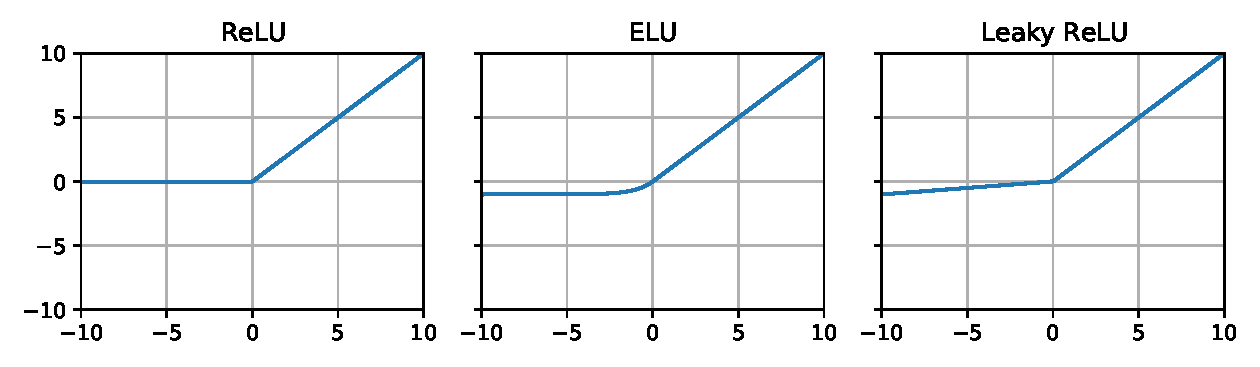
\includegraphics[width=140mm]{../../figures/03-activation-function/functions.pdf}
    \caption{Visualization of the explored activation functions. ReLU is flat in negative values and therefore has no gradient there. ELU has exponentially decaying gradient and leaky ReLU has a constant gradient. The parameter for the displayed leaky ReLU is 0.1 to make its shape more apparent.}
    \label{fig:ActivationFunctions}
\end{figure}

The convergence problems were happening at the very beginning of training. The model quickly learned to output a completely black image and never recovered from that state. We think it was an instance of the "dying ReLU" problem [CITE]. When the model is first initialized, it outputs a gray-ish image, since model weights are drawn from a uniform distribution centered on zero and the final sigmoid layer turns that into a 0.5 gray. Because the target images have black background, the model first learns to produce mostly black images. Only then does it learn to output white pixels as well (see figure \ref{fig:ActivationTrainingProgression}). With ReLU, the first training phase probably overshoots into the negative range of most synapses and that causes the model to get stuck in that negative range with zero gradient.

\begin{figure}[ht]
    \centering
    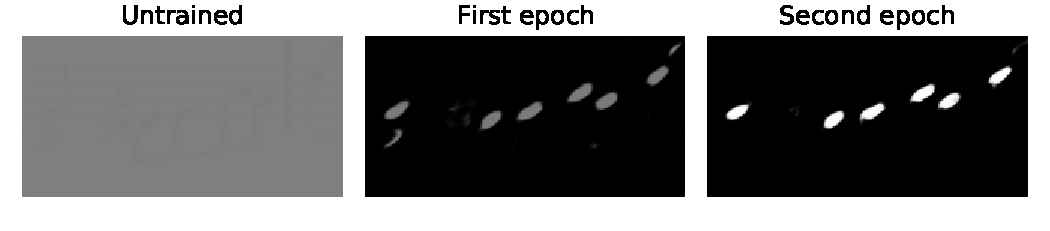
\includegraphics[width=140mm]{../../figures/03-activation-function/progression.pdf}
    \caption{The training process starts by learning to output a mostly black image, which probably causes the model to overshoot during the fully-supervised training and get stuck in the "dying ReLU" problem.}
    \label{fig:ActivationTrainingProgression}
\end{figure}

Interestingly enough, this problem happens only when training in the fully-supervised mode. We have never encountered it, when training in the semi-supervised mode. This again suggests that the unlabeled data acts as regularization, damping any extreme gradients, and stabilizing the training.

We also tried using the leaky ReLU function [CITE] with parameter $\alpha = 0.01$, however the problem still remained. Maybe a larger value for $\alpha$ would help, although we already knew that ELU works, so we haven't explored this further.

\begin{figure}[ht]
    \centering
    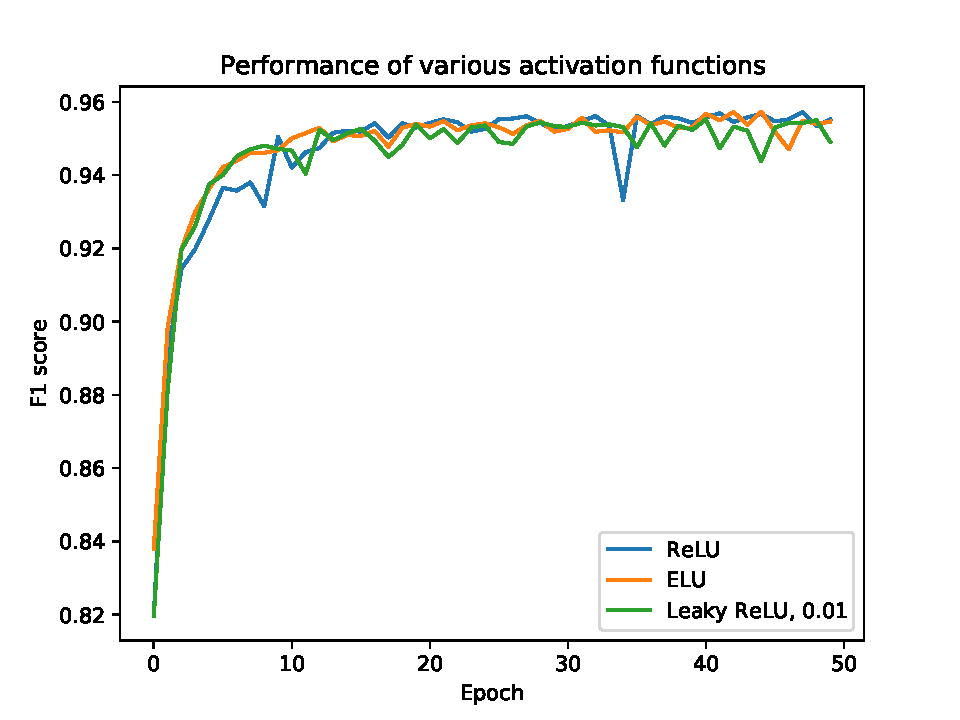
\includegraphics[width=140mm]{../../figures/03-activation-function/performance.pdf}
    \caption{An experiment from section \ref{sec:UtilizingCvcMuscima} with 8 inner features, trained in fully-supervised mode with various activation functions. All runs show the same performance.}
    \label{fig:ActivationFunctionPerformances}
\end{figure}

We run one of the experiments from section \ref{sec:UtilizingCvcMuscima} with all proposed activation functions to see what impact it has on model performance (figure \ref{fig:ActivationFunctionPerformances}). We can clearly see that they all perform equally well, so we choose ELU as the only activation function that does not suffer from the convergence problem. We thereby validate the work of Dorfer. et al. [CITE] (their article does not provide explanation for the use of ELU, but we belive they must have encountered these exact same problems).

\chapter{Conclusion and Future Work}
\label{chap:ConclusionAndFutureWork}

We have designed a scheme for training the U-Net architecture in an unsupervised manner and used it in a semi-supervised setting to try and improve optical music recognition. The unsupervised training scheme is successful at teaching the model useful representations. These are used during reconstruction to repair masked images of music sheets.

Using the model for semi-supervised learning improves training stability and the added unlabeled data regularizes the model, preventing it from overfitting. The performance of the semi-supervised model was able to reach the supervised baseline, but was unfortunately unable to surpass it.

We were also able to replicate and validate findings of other people, such as using ELU activation function to prevent the dying ReLU problem.

By looking carefully at learned reconstructions, we can see that the model produces a lot of blurred areas in places where many viable reconstructions can be generated. We belive that if a reconstruction is certain (e.g. extending stafflines), then it is not blurred. However, if a reconstruction may contain multiple viable possibilities (e.g. noteheads may have many shapes, a note can have many piches within the space of the masked area), then the model does not pick one reconstruction, but instead generates a blurred average of all of them.

We belive that replacing the simple reconstruction loss function with a discriminative network could force the model to pick a specific, realistic-looking reconstruction, instead of producing a blurred average of many reconstructions. This would reframe the reconstruction task as a generative adversarial network (GAN) problem, rather than an autoencoder problem (as it is framed now). This might be a more apropriate approach, since there is no encoded latent representation from which the image is reconstructed. It is being reconstructed out of nothing, with the only condition of matching the surrounding image.

This intuition is further supported by an article by \cite{Cuneiforms}, where the authors propose a modified GAN architecture for generating synthetic cuneiform tablets. Their model has two discriminators to force the generated tile to match the surrounding image and an auxiliary classifier that enforces generation of the correct cuneiform symbol. We would like to explore this modified scheme in a future work.

The goal of the thesis was to explore semi-supervised learning in the context of optical music recongition and to compare SSL results to a supervised baseline. We have fulfilled the goal by adapting a state-of-the-art object recognition architecture to the semi-supervised setting and evaluating it in three distinct experiments. We also explored and described all of its hyperparameters. We have not been able to surpass the supervised baseline, but we have identified possible problems and described the trajectory of our future work.


%%% Bibliography
%%% Bibliography (literature used as a source)
%%%
%%% We employ bibTeX to construct the bibliography. It processes
%%% citations in the text (e.g., the \cite{...} macro) and looks up
%%% relevant entries in the bibliography.bib file.
%%%
%%% The \bibliographystyle command selects, which style will be used
%%% for references from the text. The argument in curly brackets is
%%% the name of the corresponding style file (*.bst). Both styles
%%% mentioned in this template are included in LaTeX distributions.

\bibliographystyle{plainnat}    %% Author (year)
% \bibliographystyle{unsrt}     %% [number]

\renewcommand{\bibname}{Bibliography}

%%% Generate the bibliography. Beware that if you cited no works,
%%% the empty list will be omitted completely.

\bibliography{bibliography}

%%% If case you prefer to write the bibliography manually (without bibTeX),
%%% you can use the following. Please follow the ISO 690 standard and
%%% citation conventions of your field of research.

% \begin{thebibliography}{99}
%
% \bibitem{lamport94}
%   {\sc Lamport,} Leslie.
%   \emph{\LaTeX: A Document Preparation System}.
%   2nd edition.
%   Massachusetts: Addison Wesley, 1994.
%   ISBN 0-201-52983-1.
%
% \end{thebibliography}


%%% Figures used in the thesis (consider if this is needed)
%\listoffigures

%%% Tables used in the thesis (consider if this is needed)
%%% In mathematical theses, it could be better to move the list of tables to the beginning of the thesis.
%\listoftables

%%% Abbreviations used in the thesis, if any, including their explanation
%%% In mathematical theses, it could be better to move the list of abbreviations to the beginning of the thesis.
%\chapwithtoc{List of Abbreviations}

%%% Attachments to the master thesis, if any. Each attachment must be
%%% referred to at least once from the text of the thesis. Attachments
%%% are numbered.
%%%
%%% The printed version should preferably contain attachments, which can be
%%% read (additional tables and charts, supplementary text, examples of
%%% program output, etc.). The electronic version is more suited for attachments
%%% which will likely be used in an electronic form rather than read (program
%%% source code, data files, interactive charts, etc.). Electronic attachments
%%% should be uploaded to SIS and optionally also included in the thesis on a~CD/DVD.
%%% Allowed file formats are specified in provision of the rector no. 72/2017.
%\appendix
%\chapter{Attachments}

%\section{First Attachment}

\openright
\end{document}
